\documentclass[10pt,a4paper]{article}
\usepackage[T1]{fontenc}
\usepackage[utf8]{inputenc}
\usepackage{tgtermes,tgheros,microtype}
\usepackage[a4paper,margin=18mm,headheight=19pt]{geometry}
\usepackage{xcolor,graphicx,booktabs,tabularx,array,enumitem}
\usepackage[most]{tcolorbox}
\usepackage{fancyhdr,lastpage,titlesec}
\usepackage[hidelinks]{hyperref}
\usepackage{caption,amsmath,textcomp}

\definecolor{Navy}{HTML}{173753}
\definecolor{Teal}{HTML}{008F8C}
\definecolor{PaleTeal}{HTML}{E5F4F3}
\definecolor{Orange}{HTML}{F08A24}
\definecolor{PaleOrange}{HTML}{FFF1E2}
\definecolor{Red}{HTML}{BB3E35}
\definecolor{PaleRed}{HTML}{F9E9E7}
\definecolor{Slate}{HTML}{5B7083}
\definecolor{Green}{HTML}{2E8B57}
\definecolor{PaleGreen}{HTML}{EAF5EE}
\newcommand{\sans}{\fontfamily{qhv}\selectfont}
\newcolumntype{Y}{>{\raggedright\arraybackslash}X}
\newcolumntype{C}{>{\centering\arraybackslash}X}

\hypersetup{
  pdftitle={HeiQ XMembrane Model Closure and Material Handoff -- Revision 2},
  pdfauthor={HeiQ XMembrane project team},
  pdfsubject={Closure of the integrated ERV+EO model and experimental handoff},
  pdfkeywords={XMembrane, EO, ERV, model closure, material data, O30, break-even}
}

\pagestyle{fancy}
\fancyhf{}
\fancyhead[L]{\sans\footnotesize\color{Slate}HEIQ MATERIALS AG · XMEMBRANE}
\fancyhead[R]{\sans\footnotesize\color{Slate}MODEL CLOSURE · REVISION 2}
\fancyfoot[L]{\sans\scriptsize\color{Slate}Conditional modelling evidence · no material or product validation}
\fancyfoot[R]{\sans\scriptsize\color{Slate}Page \thepage\ of \pageref*{LastPage}}
\renewcommand{\headrulewidth}{0.45pt}
\renewcommand{\headrule}{\hbox to\headwidth{\color{Navy}\leaders\hrule height \headrulewidth\hfill}}
\titleformat{\section}{\sans\bfseries\color{Navy}\fontsize{19}{22}\selectfont}{\thesection}{0.65em}{}
\titleformat{\subsection}{\sans\bfseries\color{Navy}\fontsize{13}{16}\selectfont}{\thesubsection}{0.55em}{}
\titlespacing*{\section}{0pt}{7mm}{3mm}
\titlespacing*{\subsection}{0pt}{5mm}{2mm}
\setlength{\parindent}{0pt}
\setlength{\parskip}{1.7mm}
\setlist[itemize]{leftmargin=5mm,itemsep=1mm,topsep=1mm}
\captionsetup{font=small,labelfont={bf,color=Navy}}
\renewcommand{\arraystretch}{1.18}

\newtcolorbox{mainbox}{enhanced,breakable,colback=PaleTeal,colframe=Teal,boxrule=0.7pt,arc=2mm,left=4mm,right=4mm,top=3mm,bottom=3mm}
\newtcolorbox{warningbox}{enhanced,breakable,colback=PaleOrange,colframe=Orange,boxrule=0.7pt,arc=2mm,left=4mm,right=4mm,top=3mm,bottom=3mm}
\newtcolorbox{stopbox}{enhanced,breakable,colback=PaleRed,colframe=Red,boxrule=0.7pt,arc=2mm,left=4mm,right=4mm,top=3mm,bottom=3mm}
\newtcolorbox{gobox}{enhanced,breakable,colback=PaleGreen,colframe=Green,boxrule=0.7pt,arc=2mm,left=4mm,right=4mm,top=3mm,bottom=3mm}
\newcommand{\eyebrow}[1]{{\sans\bfseries\color{Teal}\MakeUppercase{#1}}\par\vspace{1.5mm}}

\begin{document}
\thispagestyle{empty}
\vspace*{8mm}
\begin{tcolorbox}[enhanced,colback=Navy,colframe=Navy,boxrule=0pt,arc=0mm,left=12mm,right=12mm,top=12mm,bottom=12mm]
{\sans\bfseries\large\color{white}HEIQ XMEMBRANE PROJECT TEAM}\par
\vspace{8mm}
{\sans\bfseries\fontsize{28}{32}\selectfont\color{white}Model closure and\\[-1mm]material handoff}\par
\vspace{2mm}
{\sans\fontsize{18}{21}\selectfont\color{white}What the integrated ERV+EO model has established}\par
\vspace{7mm}
{\sans\large\color{white}31 August 2026\quad · \quad Revision 2}
\end{tcolorbox}

\vspace{10mm}
{\sans\bfseries\Large\color{Navy}Controlled correction to the earlier closure note}\par
\vspace{4mm}
This revision uses the selected architecture only: EO is integrated in the
ERV membrane/core. It supersedes the earlier closure report wherever that
report described a downstream or post-ERV EO module, used the historical
180-Wh/kg shorthand as break-even, or attributed an AC-only difference to EO.

\begin{mainbox}
\textbf{Closure in one sentence.} The equations, signed transport audit and
matched architecture comparison are internally consistent and identify an
O30 opportunity below 9,000~m\textsuperscript{2}; the remaining uncertainty is
not another algebraic degree of freedom, but measured material coupling and
the omitted receiver, heat-rejection, conversion and hardware power.
\end{mainbox}

\vfill
\begin{tabularx}{\textwidth}{@{}lY@{}}
\textbf{Fixed service} & O80 at 32~$^\circ$C/80\% RH to 20~$^\circ$C/50\% RH supply \\
\textbf{Selected point} & Integrated ERV+EO to O30; 5,899~m\textsuperscript{2}; 418.400~kW known subtotal \\
\textbf{Passive control} & Same ERV with EO off plus AC: 543.741~kW \\
\textbf{Incremental window} & 125.340~kW or 23.05\% versus the passive control \\
\textbf{Calculated break-even} & 51.955~Wh/kg all-in active-core energy \\
\textbf{Claim boundary} & Conditional model window; no validated membrane, module or net-system saving \\
\end{tabularx}

\clearpage
\section{What ``model closure'' means}
\eyebrow{The model question is closed; the material question is deliberately open}

Model closure does not mean that a product has been validated. It means that
the previously ambiguous definitions, signs, comparators and decision
coordinates have been made explicit enough that the model gives reproducible
answers and exposes the measurements that now control the decision.

\begin{tabularx}{\textwidth}{@{}p{0.26\textwidth}YY@{}}
\toprule
\textbf{Question} & \textbf{Closed result} & \textbf{What remains open} \\
\midrule
Where EO acts & Inside the ERV membrane/core only & Core construction and current collection \\
What O50/O30 mean & Intermediate humidity-ratio targets, not supply-air states & Measured achievable outlet under real films \\
What EO is compared with & Same passive ERV+AC system with EO off & Full-system parasitic ledger \\
Whether O50 needs EO & No; passive ERV already reaches 13.215~g/kg, below O50 at 14.952~g/kg & Sensitivity to measured exchanger performance \\
Whether O30 fits the area gate & Yes in the screened model: 5,899~m\textsuperscript{2} at 1.00~V & Manufacturable packing and pressure drop \\
Whether full EO drying fits & No; the minimum valid screened full-duty area is about 17,253~m\textsuperscript{2} & No further claim below 9,000~m\textsuperscript{2} \\
\bottomrule
\end{tabularx}

The thermodynamic audit also closes the sign convention. A locally positive
passive surface direction is not a rejection criterion for electrically
driven transport against that passive tendency. Feasibility is tested with
the total electrochemical driving force and entropy-production sign, not by
requiring the passive water-activity gradient to point in the desired pumping
direction.

\begin{warningbox}
The phrase ``no primary row resolves the local surface direction'' meant that
the screened literature or property rows did not independently determine the
sign and magnitude of the membrane-surface water-activity gradient under the
actual ERV film conditions. That absence prevents material ranking from that
single gradient; it does not invalidate active uphill EO transport.
\end{warningbox}

\section{Energy closure for the integrated architecture}
\eyebrow{The break-even is calculated from the matched passive control}

For the selected O30 point, the integrated core removes
4,365.918~kg/h of water. The remaining AC load is 316.910~kW. The maximum
all-in active-core specific energy that preserves parity with the same passive
ERV+AC control is therefore
\[
e_{\mathrm{BE}}=
\frac{543.741-316.910}{4{,}365.918/3{,}600}
=51.955~\mathrm{Wh/kg}.
\]
The known active-core term is 101.490~kW, or 23.246~Wh/kg. The difference is
28.709~Wh/kg, equivalent to 125.340~kW. This is the complete remaining budget
for the loads omitted from the present subtotal.

\begin{figure}[htbp]
  \centering
  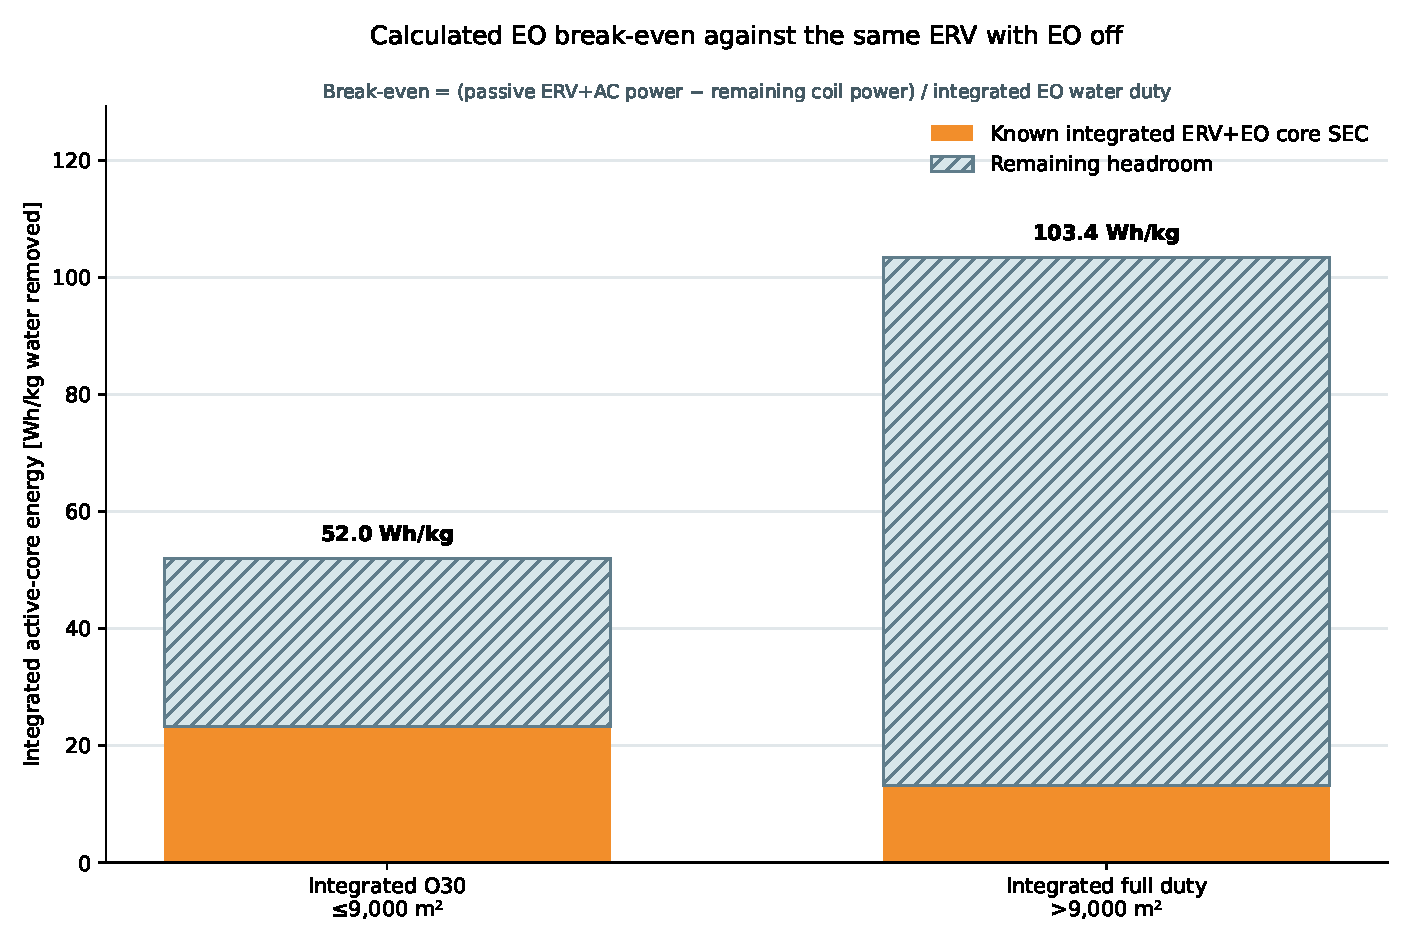
\includegraphics[width=0.94\textwidth]{figures/integrated_break_even_sec.pdf}
  \caption{Architecture-specific break-even. The historical 180-Wh/kg value is not used as the selected break-even.}
\end{figure}

\begin{stopbox}
\textbf{No net-saving claim yet.} Receiver work, heat rejection, conversion
losses, electrodes, current collection, manifold losses, incremental fan
power, leakage and durability are not all closed. Their combined O30 load
must remain below 125.340~kW for the conditional incremental advantage to
survive.
\end{stopbox}

\clearpage
\section{What was learned about membrane selection}
\eyebrow{There is no valid single-property winner}

The model rejects selection by water diffusivity alone. The EO response and
power depend on a coupled property bundle evaluated at the same temperature,
water activity, mechanical compression and electrode state:
\[
\left\{
\frac{D_w}{L}\frac{\partial C_w}{\partial a_w},\;
n_{\mathrm{drag}},\;
\sigma_{\mathrm{wet}},\;
ASR_{\mathrm{compressed}},\;
L,\; C_w(a_w),\; \text{mechanical stability}
\right\}.
\]
High sorption or diffusivity may improve passive permeation while low wet
conductivity or high compressed resistance raises electrical loss. Likewise,
large electro-osmotic drag is not useful if current must pass through an
unacceptably resistive wet membrane. The properties must therefore be
measured as a joint vector on the same sample, not assembled from unrelated
best values.

\subsection{Symmetry and Yaroshchuk-type asymmetry}

The current model includes a symmetric quasi-static $+J/0/-J$ replay. Under
the present constant-drag constitutive law, the positive- and negative-current
contributions cancel around the passive state, producing no useful mean EO
pumping. The study has \textbf{not} yet implemented a validated asymmetric
Yaroshchuk-style membrane, rectifying interfaces, direction-dependent drag or
memory. Such an effect could change the cycle mean, but only after its
constitutive relation and parameters are supplied by measurement or a
traceable source.

\begin{mainbox}
\textbf{Material handoff requirement.} Measure on the same conditioned coupon:
sorption isotherm and derivative, water mobility/permeance, EO drag versus
current and polarity, wet conductivity, compressed ASR, thickness, swelling,
gas permeability and mechanical response. Preserve raw polarity-resolved
transients so asymmetry can be tested rather than assumed.
\end{mainbox}

\section{Experimental closure route}
\eyebrow{A controlled-flow coupon cell can falsify the model assumptions}

The recommended first fixture is a two-sided controlled-flow vapour cell with
a 50$\times$50-mm active aperture (25~cm\textsuperscript{2}), approximately
80$\times$80-mm coupon and 110$\times$110-mm outer plates. Use interchangeable
symmetric 1/2/4-mm flow gaps, with 2~mm nominal. At 1~m/s the nominal actual
flow is 6.0~L/min per side. Start with 8--10-mm insulating flow frames and
12-mm metal backing/load plates; a load-bearing PEEK plate should start near
16~mm and be accepted only after loaded flatness and gap mapping.

The required controls are a split common inlet, EO-off/EO-on ABBA sequencing,
two-sided water balance, foil blank, polarity reversal, pressure control,
gap/flow repeats, reference cross-switching and multiple perimeter inserts.
Closed chambers are acceptable only as transient inventory tests; they must
not be interpreted as fixed-boundary steady-state measurements.

\begin{figure}[htbp]
  \centering
  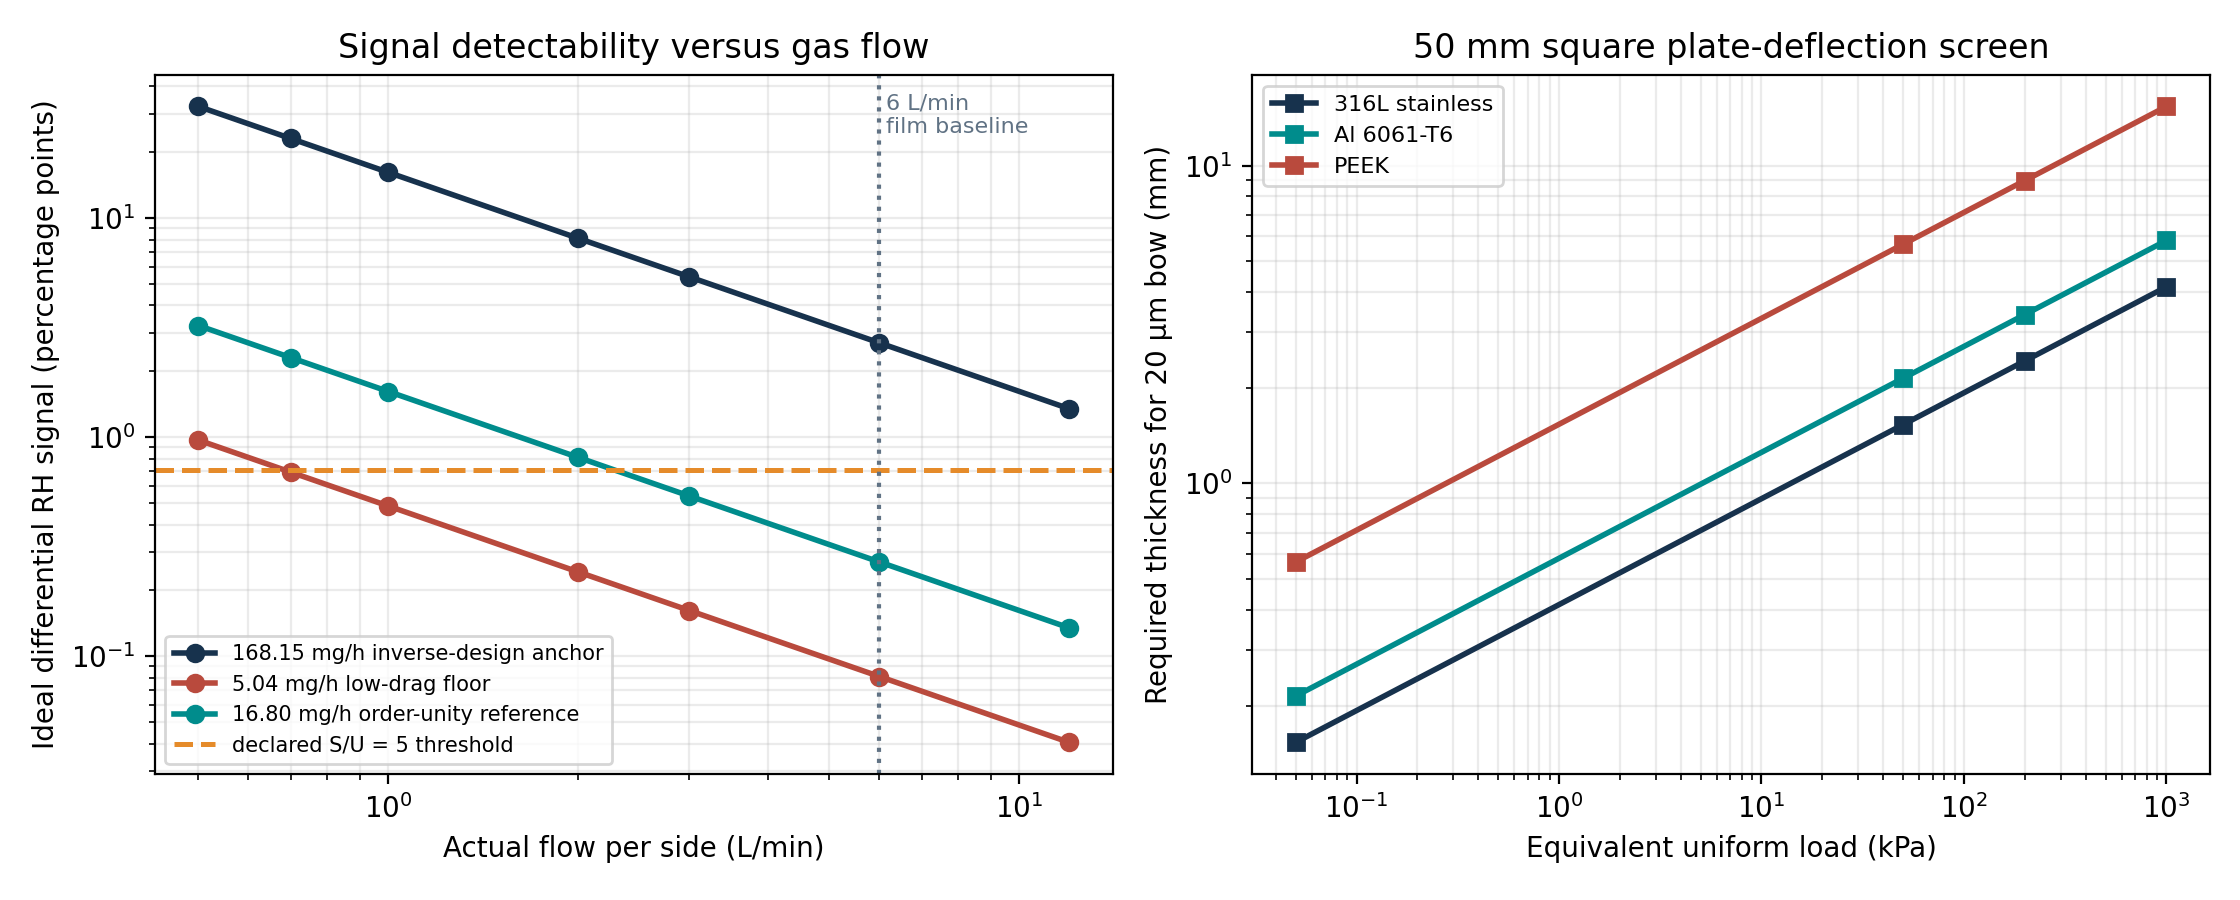
\includegraphics[width=0.94\textwidth]{figures/cell_dimension_tradeoffs.png}
  \caption{Coupon-cell sizing and detectability trade-offs for the recommended starting fixture.}
\end{figure}

\clearpage
\section{Decision and completion criteria}
\eyebrow{The correct next step is evidence generation, not another unconstrained sweep}

\begin{tabularx}{\textwidth}{@{}Yp{25mm}Y@{}}
\toprule
\textbf{Decision} & \textbf{Status} & \textbf{Reason} \\
\midrule
Use passive ERV as the primary control & \textcolor{Green}{\textbf{GO}} & Established matched reduction to 543.741~kW \\
Test EO integrated in ERV to O30 & \textcolor{Green}{\textbf{GO}} & 5,899~m\textsuperscript{2}; 125.340-kW conditional window \\
Assign EO duty to O50 & \textcolor{Slate}{\textbf{NO DUTY}} & Passive ERV already passes O50 \\
Claim full EO drying below 9,000~m\textsuperscript{2} & \textcolor{Red}{\textbf{NO-GO}} & Minimum valid screened area is about 17,253~m\textsuperscript{2} \\
Claim measured net energy saving & \textcolor{Orange}{\textbf{NOT YET}} & Omitted subsystem ledger remains open \\
Select a commercial membrane & \textcolor{Orange}{\textbf{NOT YET}} & Same-sample coupled properties are unmeasured \\
Build the controlled-flow coupon fixture & \textcolor{Green}{\textbf{GO}} & Dimensions, controls and error mechanisms are defined \\
\bottomrule
\end{tabularx}

\begin{gobox}
\textbf{Model-phase conclusion.} The model is sufficiently closed to stop
unfocused parameter exploration and proceed to a matched EO-off/EO-on coupon
campaign. The O30 opportunity survives only if measured active-core behaviour
and the complete omitted-load ledger remain below the calculated
51.955-Wh/kg break-even. The next decision is empirical, not cosmetic.
\end{gobox}

\section*{Controlled evidence basis}

This report is subordinate to the Version~9 final result and decision report.
Its numerical evidence is reproduced from the integrated active-core case
register, the under-9,000-m\textsuperscript{2} selection register, the matched
opportunity plots and the vapour-cell sizing and boundary-condition analyses
included in the controlled Version~9 release package.

\vfill
{\sans\scriptsize\color{Slate}End of Model Closure and Material Handoff, Revision 2. This document contains conditional modelling and experiment-planning results; it is not a product-performance certificate.}

\end{document}
